\documentclass{article}

\usepackage{amssymb}
\usepackage{amsmath}
\usepackage{amsthm}
\usepackage{algorithm}
\usepackage{graphicx}
\usepackage{caption}
\usepackage{fullpage}
\usepackage{cmap}
\usepackage{enumerate}
\usepackage{algorithm}
\usepackage{algorithmic}
\usepackage{float}
\usepackage{subfigure}
\usepackage{color}
\usepackage{amssymb}
\usepackage{listings}


\makeatletter
\newcommand{\leqnomode}{\tagsleft@true}
\newcommand{\reqnomode}{\tagsleft@false}
\DeclareMathOperator*{\argmax}{argmax}
\DeclareMathOperator*{\argmin}{argmin}
\DeclareMathOperator*{\softmax}{softmax}
\makeatother

% THEOREMS -------------------------------------------------------
\newtheorem{theorem}{Theorem}[section]
\newtheorem{corollary}[theorem]{Corollary}
\newtheorem{lemma}[theorem]{Lemma}
\newtheorem{observation}[theorem]{Observation}
\newtheorem{proposition}[theorem]{Proposition}
\newtheorem{claim}[theorem]{Claim}
\newtheorem{fact}[theorem]{Fact}
\newtheorem{assumption}[theorem]{Assumption}

\theoremstyle{definition}
\newtheorem{definition}[theorem]{Definition}
\theoremstyle{remark}
\newtheorem*{remark}{Remark}
\newtheorem{example}{Example}
\numberwithin{equation}{section}


\setlength{\parindent}{0pt}
% ----------------------------------------------------------------
\begin{document}

\title{CS 224N: Homework 3}
\author{Chen Qian (cqian23@stanford.edu)\\
Tianchang He (th7@stanford.edu)\\
Rao Zhang (zhangrao@stanford.edu)}
\date{}
\maketitle
% ----------------------------------------------------------------

\section*{Question 1}

(a) 
i. \\
(1) How much do you know about Washington? (here Washington can either refer to the president or the state)

(2) You should ask Google for help. (here Google can either refer to the company or the search engine)
 
 \vspace{10pt}
 
 ii. To include the meaning of context, which could somewhat eliminate the ambiguity of a word.
 
 \vspace{10pt}
 
 iii. Constituency; Dependency; Location of the word.
 
 \newpage
 (b) 
 
 i.
 
 $e^{(t)}$: 1 * (2w + 1) D \\
 $W$: (2w + 1) D * H \\
 $U$: H * C.
 
 ii.
 
 For each window, the computational complexity is: 
 \begin{align*}
 T &=  T(\text{compute} \quad e^{t})  + T(\text{compute}  \quad h^{t}) +  T(\text{compute} \quad  \hat{y}^{t}) \\
    &= O((2w + 1)D) + O((2w + 1) D * H) + O(H*C) \\
    &= O ( wD * H + H *C ).
 \end{align*}
Notice that $x^{t}$ is a one-hot vector, so $x^{t}L$ takes $O(D)$ instead of $O(V*D)$ time.

Thus, for a sentence of length $T$, the computational complexity is $O ( T (w D * H + H *C) )$.


\newpage
 (d)
 
 i.
 
 \begin{figure}[H] 
  \centering
 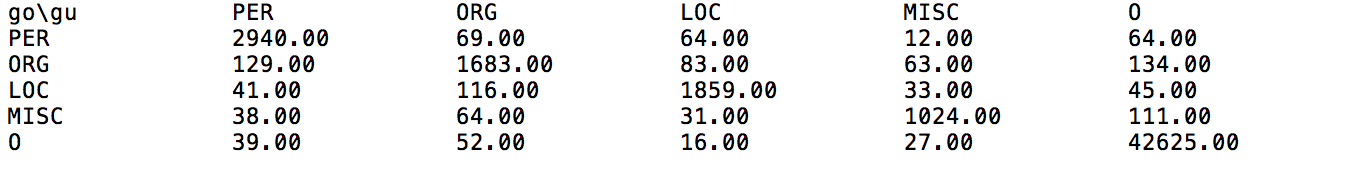
\includegraphics[width=100mm, height=20mm]{fig/token-level-confusion.png}
   \caption{token-level confusion matrix}
   \label{fig: confuse}
 \end{figure}
 
 The best F1 score is 84\%. The confusion matrix is shown in Fig. \ref{fig: confuse}. According to the confusion matrix, we claim that Person entity is likely to be classified as Organization, and Organization and Location are likely to be misclassified as each other.
 
 ii.
 
  \begin{figure}[H] 
  \centering
 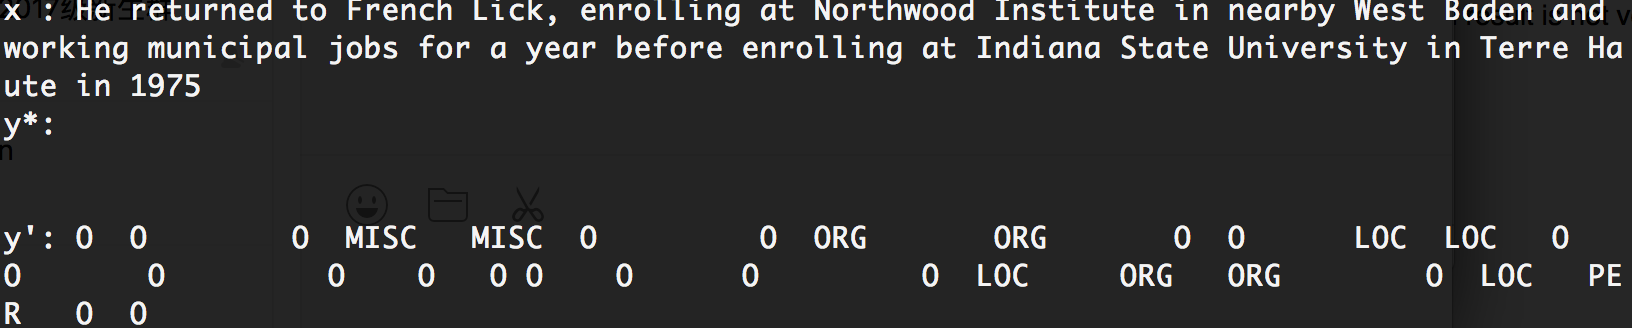
\includegraphics[width=100mm, height=20mm]{fig/eg1.png}
   \caption{The example for limitation 1}
   \label{fig: eg1}
 \end{figure}
 
 Limitation 1: The performance of this window-based model is largely impacted by the size of window. For words in sentences longer than the window size, the classification result is not very accurate. The example is shown in Fig. \ref{fig: eg1}.
 
 
 \begin{figure}[H] 
  \centering
 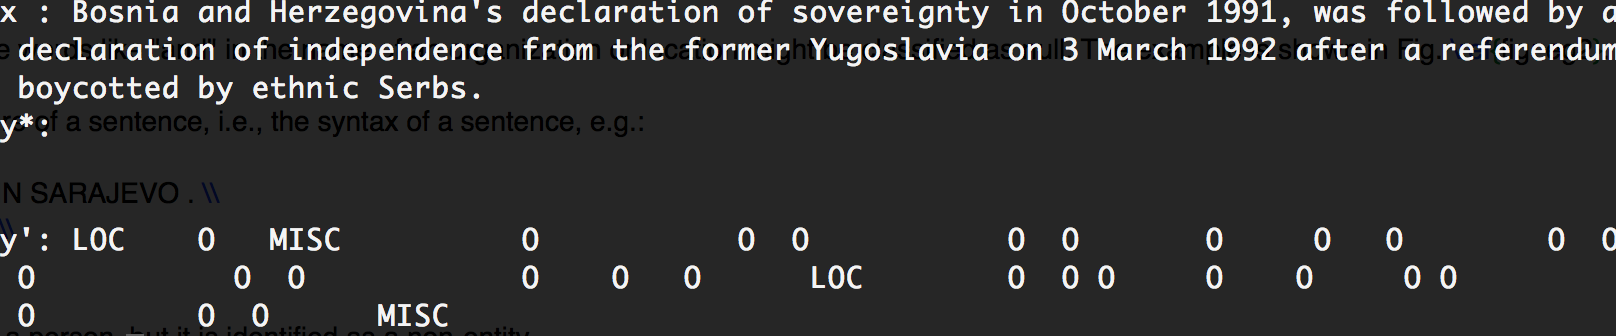
\includegraphics[width=100mm, height=20mm]{fig/eg2.png}
   \caption{The example for limitation 2}
   \label{fig: eg2}
 \end{figure}
 
 Limitation 2: Words are examined individually, so some words like "and" in the name of an organization or location might be classified as null. The example is shown in Fig. \ref{fig: eg2}.
 
 Limitation 3: The model somewhat ignores the structure of a sentence, i.e., the syntax of a sentence, e.g.:
 
x : ATHLETICS - HARRISON , EDWARDS TO MEET IN SARAJEVO . \\
y*: O         O PER      O PER     O  O    O  LOC      O   \\
y': O         O O        O ORG     O  O    O  LOC      O   \\

Due to the structure/syntax, Harrison is and should be a person, but it is identified as a non-entity. 


\newpage

\section*{Question 2}

(a) 

i. In RNN, we add a new parameter matrix $W_h$, whose dimension is $H * H$. Thus, RNN has $H * H$ parameters than window-based model.

\vspace{10pt}

ii. Recalling that RNN at a time takes one word as the input, and outputs the prediction. Thus, we only need to compute the computational complexity of one turn, and the total time is just the result times T. The time for one turn is:
 \begin{align*}
 T &=  T(\text{compute} \quad e^{t})  + T(\text{compute}  \quad h^{t}) +  T(\text{compute}  \quad  \hat{y}^{t}) \\
    &= O(D) + O( D * H + H * H)  +  O(H*C) \\
    &= O ( D * H + H *C + H * H ).
 \end{align*}
 
 
Hence, the total computational complexity is $O ( T  (D * H + H *C + H * H) )$.

\newpage

(b) 

i. For example, if we have two words x and y, separately of Person label and null label. Initially, the probability of classifying $x$ as Person is $0.3$, which is the maximal among all categories, and the probability of classifying $y$ as null is also $0.3$, which is also the maximal. In this case, the F1 score is $\frac{2}{1 + 1} = 1$. Then, by some way, we keep the probability of classifying $x$ as Person being $0.3$, but no longer the maximal among all categories, and increase the the probability of classifying $y$ as null to $0.5$. In the new case, cross-entropy loss decreases from $-2\log0.3$ to $-\log0.5$, but the F1 score across classes drops to 0.5. This can happen on a minibatch and we cannot optimize the weights based on F1 score (which is a macroscopic and discrete evaluation).

\vspace{10pt}

ii. Because F1 score is not continuous. Thus, if we use F1 score as the loss function, then we cannot compute the gradients of parameters.

\newpage


(d)

The loss will be larger because we take more items into account, and gradient updates will be noisy because we compute gradients on some meaningless data. If masking is applied, for $t > T$. $m^{(t)}$ is 0. Thus,  when computing loss and gradients, complementary words will not be considered, so it solves the problem.
 
 \newpage
 (g) 
 
 i. 
 
  \begin{figure}[H] 
  \centering
 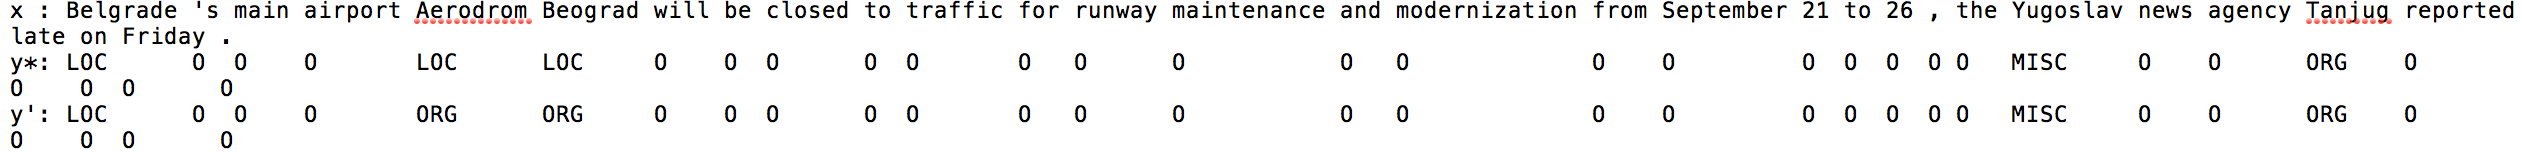
\includegraphics[width=120mm, height=10mm]{fig/eg3.png}
   \caption{The example for limitation 2}
   \label{fig: eg3}
 \end{figure}
 
  \begin{figure}[H] 
  \centering
 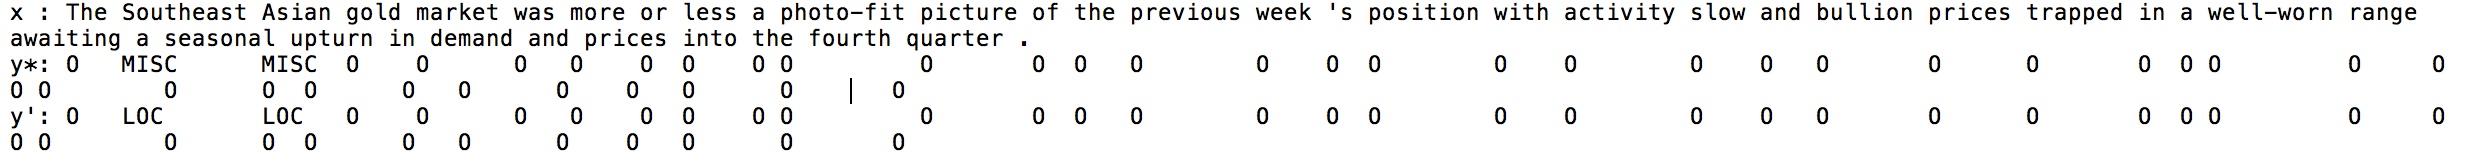
\includegraphics[width=120mm, height=10mm]{fig/eg4.png}
   \caption{The example for limitation 2}
   \label{fig: eg4}
 \end{figure}
 
 
 Limitation 1: RNN cannot take future words into consideration. The example is shown in Fig. \ref{fig: eg3}.
 
 Limitation 2: RNN suffers from gradients vanishing. The example is shown in Fig. \ref{fig: eg4}.
 
 ii.
 
 Solution 1: Use bi-directional network instead.
 
 Solution 2: Use GRU units instead.
 
 
 \newpage
 
 \section{Question 3}
 
 (a) 
 
 i.
 
$w_h = 1, u_h = 1, b_h = -0.5$.

ii. There are many possible solutions, let us provide one as the following:

$u_z = 1, w_z = 1, u_h = 1, w_h = 0$.

\newpage

(b) 

i. Assume that RNN cell could replicate the behavior, there must be the following equations:
\begin{align*}
&u_h  + b_h > 0 \\
&u_h + w_h + b_h < 0 \\
&w_h + b_h > 0 \\
&b_h < 0.
\end{align*}

These 4 equations separately correspond to:

(1) h = 0, x = 1, jump to h = 1. 

(2) h = 1, x = 1, jump to h = 0. 

(3) h = 1, x = 0, maintain h = 1. 
 
(4) h = 0, x = 0, maintain h = 0. 

Since $b_h < 0$ and $u_h  + b_h > 0$, we have $u_h > 0$. We also have $w_h + b_h > 0$, so there must be $u_h + w_h + b_h > 0$, which is contradictory to the second equation. Thus, we claim that RNN cell cannot replicate the behavior.

\vspace{10pt}

ii.

There are still many candidate solutions, we provide one as the following:

$b_r = 1, w_z = 1, u_z = -1, u_h = 1, w_h = -2$.

\newpage
(d)

 \begin{figure}[H] 
  \centering
 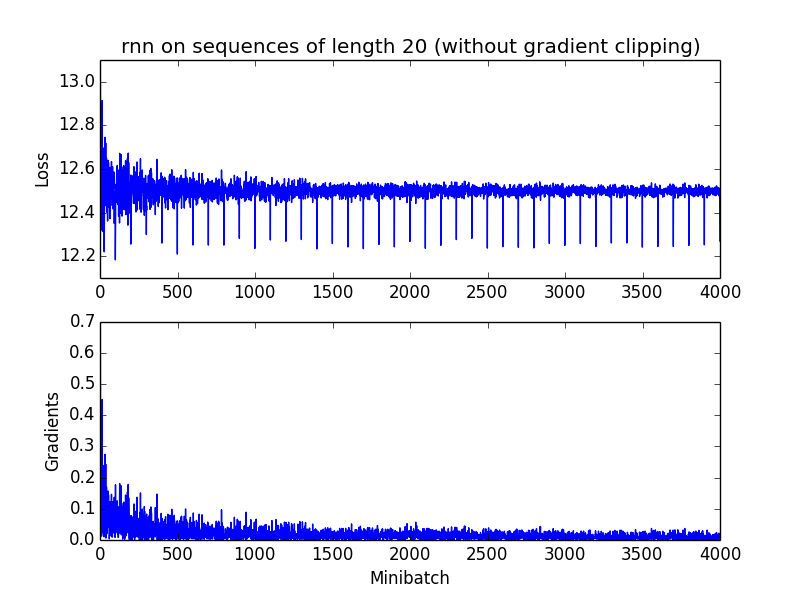
\includegraphics[width=100mm, height=70mm]{fig/q3-noclip-rnn.png}
   \caption{}
   \label{fig: noclip_rnn}
 \end{figure}
 
  \begin{figure}[H] 
  \centering
 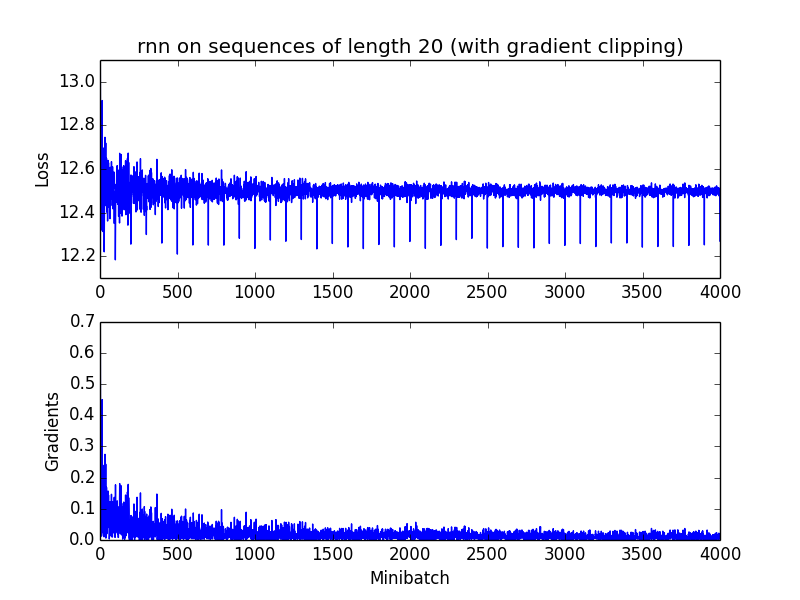
\includegraphics[width=100mm, height=70mm]{fig/q3-clip-rnn.png}
   \caption{}
   \label{fig: clip_rnn}
 \end{figure}
 
  \begin{figure}[H] 
  \centering
 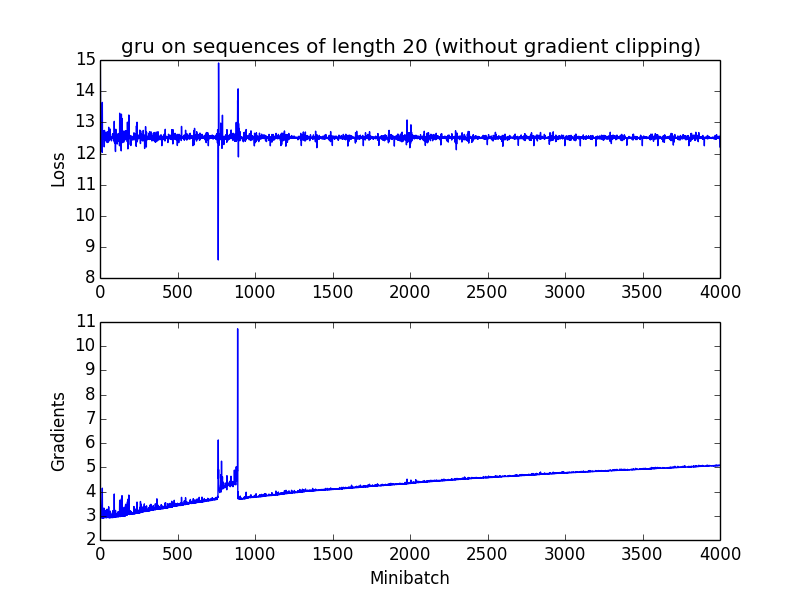
\includegraphics[width=100mm, height=70mm]{fig/q3-noclip-gru.png}
   \caption{}
   \label{fig: noclip_gru}
 \end{figure}
 
  \begin{figure}[H] 
  \centering
 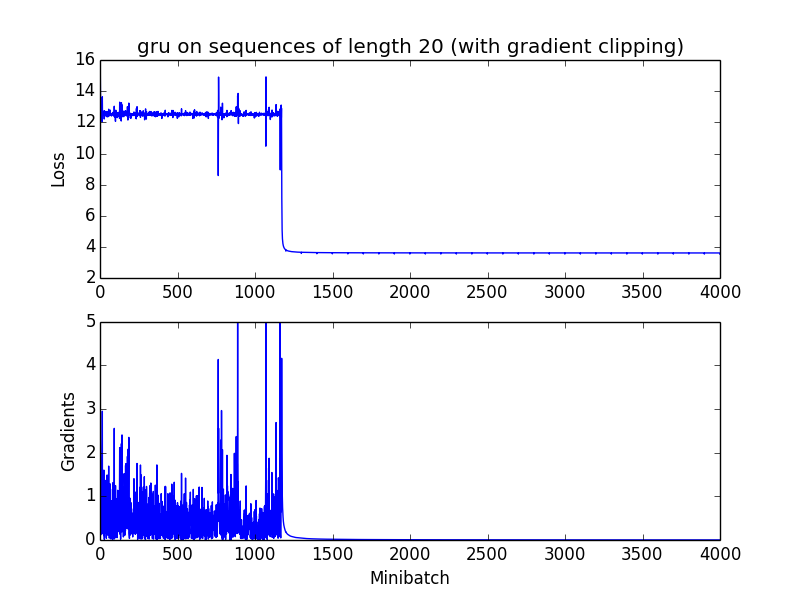
\includegraphics[width=100mm, height=70mm]{fig/q3-clip-gru.png}
   \caption{}
   \label{fig: clip_gru}
 \end{figure}
\newpage
(e)\\
 i. There is exploding gradient problem in GRU if we do not apply clipping, and clipping helps solve the problem. Also, there is vanishing gradient problem in rnn and clipping won't do much.
 
 \vspace{10pt}
 
 ii. Comparing the loss of GRU and RNN we can conclude that GRU works better than RNN. Because GRU keeps around memories to capture long distance dependencies. 
 
\end{document}